\documentclass[12pt]{beamer}
\usetheme{CambridgeUS}
\usepackage[utf8]{inputenc}
\usepackage[spanish]{babel}
\usepackage{amsmath}
\usepackage{amsfonts}
\usepackage{amssymb}
\usepackage{graphicx}
\author{Kevin García - Alejandro Vargas}
\title{Multicolinealidad}
%\setbeamercovered{transparent} 
%\setbeamertemplate{navigation symbols}{} 
%\logo{} 
%\institute{} 
%\date{} 
%\subject{} 
\begin{document}

\begin{frame}
\titlepage
\end{frame}

%\begin{frame}
%\tableofcontents
%\end{frame}
\begin{frame}
\frametitle{Introducción}
~\\ En esta presentación evaluaremos la presencia de multicolinealidad en el modelo lineal ajustado para los 500 datos seleccionados de la base de datos 'cadata'. Se dará una presentación formal de la multicolinealidad y se mostraran algunas consecuencias que tiene la presencia de este, además, se describirán y se aplicarán distintos métodos para verificar la presencia o ausencia de esta en nuestro modelo lineal ajustado, posteriormente se tratara de solucionar esto, llevando a cabo estimación por PCR(regresión por componentes principales) y finalmente, se concluirá acerca del modelo teniendo en cuenta los resultados de los métodos aplicados y de la estimación por PCR comparada con los estimadores por MCO(mínimos cuadrados ordinarios) .
\end{frame}

\begin{frame}
\frametitle{Modelo planteado}
~\\ El modelo sobre el cuál se va a evaluar la presencia de la multicolinealidad, es el modelo que se planteó en la tarea 1, que pretendía explicar la variable 'Valor mediano de las viviendas' con las variables explicativas 'Ingreso mediano','Edad mediana de la vivienda','Total de habitaciones','Total de dormitorios','Población' y 'Hogares'. El modelo planteado para estas variables, sin hacer transformación ni selección de estas es:
$$ValorMediano =\beta_{0}+\beta_{1}(IngresoMediano)+\beta_{2}(EdadMediana)+\beta_{3}(TotalDeHabitaciones)$$
$$+\beta_{4}(TotalDeDormitorios)+\beta_{5}(Poblacion)+\beta_{6}(Hogares) $$
\end{frame}

\begin{frame}
\frametitle{Multicolinealidad}
~\\La multicolinealidad implica una dependencia casi lineal entre los regresores, los cuales son las columnas de la matriz X, por lo que es claro que una dependencia lineal exacta causaría una matriz $X^{T}X$ singular. La presencia de dependencias casi lineales puede influir en forma dramática sobre la capacidad de estimar coeficientes de regresión afectando la precisión de las estimaciones. Cuando existe multicolinealidad en nuestro modelo, el análisis por mínimos cuadrados puede ser totalmente inadecuado.
\end{frame}

\begin{frame}
\frametitle{Posibles causas de la multicolinealidad}
~\\La multicolinealidad se puede dar por cuatro fuentes principales:
\begin{itemize}
\item[1.]]El método de recolección de datos que se empleó:Puede originar problemas de multicolinealidad cuando el analista sólo muestrea un subespacio de la región de los regresores definidos.
\item[2.]Restricciones en el modelo o en la población:Las restricciones en el modelo o en la población que se muestrea pueden causar multicolinealidad; por ejemplo, supóngase que una empresa eléctrica está investigando el efecto del ingreso familiar $(X_{l})$ y el tamaño de la vivienda $(X_{2})$ sobre el consumo eléctrico residencial.En este ejemplo, una restricción física en la población fue lo que causó este fenómeno: las familias que tienen ingresos mayores en general tienen casas mayores que las familias de menores ingresos, cuando hay restricciones físicas como ésta, habrá multicolinealidad independientemente del método de muestreo que se emplee.
\end{itemize}
\end{frame}

\begin{frame}
\frametitle{Posibles causas de la multicolinealidad}
\begin{itemize}
\item[3.]Especificación del modelo:También se puede inducir la multicolinealidad por la elección del modelo. Por ejemplo,al agregar términos polinomiales a un modelo de regresión se produce un deterioramiento en $X^{T}X$, además, si el rango de X es pequeño, al agregar un término en $X^{2}$ puede producirse una multicolinealidad importante. 
\item[4.]Un modelo sobredefinido:Cuando se tienen mas variables regresoras que observaciones se puede generar un problema de multicolinealidad.
\end{itemize}
\end{frame}


\begin{frame}
\frametitle{Consecuencias de la multicolinealidad}
~\\Una multicolinealidad fuerte entre los regresores del modelo,da como resultado grandes varianzas y covarianzas de los estimadores de coeficientes de regresión por mínimos cuadrados.Esto implica que distintas muestras tomadas con los mismos valores de X podrían ocasionar estimaciones muy diferentes de los parámetros del modelo.
\end{frame}

\begin{frame}
\frametitle{Métodos para detectar multicolinealidad}
~\\Para detectar la multicolinealidad se utilizaran los 4 métodos de diagnostico expuestos en el libro de montgomery, que son los siguientes:
\begin{itemize}
\item[1.]Examen de la matriz de correlación:Una medida muy sencilla de la multicolinealidad es la inspección de los elementos $r_{ij}$ no diagonales en la matriz de correlaciones. Si los regresores $x_{i}$ y $x_{j}$ son casi linealmente dependientes $|r_{ij}|$ será próximo a 1. Para nuestros datos, la matriz de correlaciones es la siguiente:
\end{itemize}
\end{frame}

\begin{frame}
\frametitle{Métodos para detectar multicolinealidad}

\[R=
\left( \begin{array}{cccccc}
 1 & 0.01725 & 0.07903 & -0.18136 & -0.16257 & -0.16049 \\ 
   & 1       & -0.31169& -0.17024 & -0.26517 & -0.14456 \\
   &         & 1       & 0.86207  & 0.85768  & 0.86527 \\
   &         &         & 1        & 0.83406  & 0.98870 \\
   &         &         &          & 1        & 0.85391 \\
   &         &         &          &          & 1
\end{array} \right) \]
~\\La matriz de correlaciones R, nos muestra perfectamente la alta correlación que existe entre las últimas 4 variables regresoras o explicativas (Total de habitaciones, total de dormitorios, población y hogares) , por lo cuál es casi evidente que una o varías de estas sobran en el modelo y pueden ocasionar multicolinealidad.
\end{frame}

\begin{frame}
\frametitle{Métodos para detectar multicolinealidad}
\begin{itemize}
\item[2.]Factores de inflación de varianza:Como la varianza de los j-ésimos coeficientes de regresión es $C_{jj}\sigma^2$ se puede considerar que $C_{jj}$ es el factor en el que aumenta la varianza de $\hat{\beta_{j}}$ debido a dependencias casi lineales entre los regresores.
~\\Entonces se define el factor de inflación de varianza como: 
$$VIF_{j}=C_{jj}=(1-R^2_{j})^{-1}$$
~\\El factor VIF (de variance inflation factor) para cada término del modelo mide el efecto combinado que tienen las dependencias entre los regresores sobre la varianza de ese término. Si hay uno o más VIF grandes, hay multicolinealidad. El criterio dice que si cualquiera de los VIF es mayor que 5 o 10, es indicio de que los coeficientes asociados de regresión están mal estimados debido a la multicolinealidad.
\end{itemize}
\end{frame}

\begin{frame}
\frametitle{Métodos para detectar multicolinealidad}
~\\Los $VIF_{i}$ para este modelo son:
~\\\begin{tabular}{llllllll}
\hline 
VARIABLE & Ing.Mediano & Edad Mediana & T.Habitaciones & T.Dormitorios & Población & Hogares \\ 
\hline 
VIF & 1.565795 & 1.271698 & 8.203393 & 52.2694 & 5.675371 & 56.12648 & \\ 
\hline 
\end{tabular} 
~\\Podemos ver que hay 2 VIF mayores que 5 y 2 VIF mayores que 10, entonces podemos afirmar que los coeficientes de regresión asociados a estas variables están mal estimados debido a la multicolinealidad.
\end{frame}

\begin{frame}
\frametitle{Métodos para detectar multicolinealidad}
\begin{itemize}
\item[3.]Análisis del eigensistema de $X^{T}X$:Los valores propios de $X^{T}X$, por ejemplo $\lambda_{1},\lambda_{2},...,\lambda_{p}$ se pueden usar para medir el grado de multicolinealidad en los datos. Si hay una o más dependencias casi lineales en los datos, una o más de las raíces características será pequeña. Uno o más eigenvalores pequeños implican que hay dependencias casi lineales entre las columnas de X. Algunos analistas prefieren examinar el número de condición de $X^{T}X$, que se define como $k=\frac{\lambda_{max}}{\lambda_{min}}$
~\\En general, si el número de condición es menor que 100, no hay problema grave de multicolinealidad. Los números de condición de 100 a 1 000 implican multicolinealidad de moderada a fuerte, y si k es mayor que 1 000, es indicio de una fuerte multicolinealidad.
\end{itemize}
\end{frame}

\begin{frame}
\frametitle{Métodos para detectar multicolinealidad}
~\\Los indices de condición de la matriz $X^{T}X$ son
~\\$$k_{j}=\frac{\lambda_{max}}{\lambda_{j}} ; j=1,2,...,p$$
~\\La cantidad de indices de condición que son grandes (digamos, $\geq 1000$) es una medida útil de la cantidad de dependencias casi lineales en $X^{T}X$.
~\\Los valores propios para la matriz $X^{T}X=R$ (en forma de correlación) correspondiente a nuestros datos son:
~\\$\lambda_{1}=3.72181333,\lambda_{2}=1.05255886,\lambda_{3}=0.93404888,\lambda_{4}=0.19394997,\lambda_{5}=0.08822446,\lambda_{6}=0.00940450$
\end{frame}

\begin{frame}
\frametitle{Métodos para detectar multicolinealidad}
~\\De aquí, tenemos que $\lambda_{max}=3.72181333$ y $\lambda_{min}=0.00940450$, por lo tanto el número de condición es:
$$k=\frac{\lambda_{max}}{\lambda_{min}}=\frac{3.72181333}{0.00940450}=395.7481344$$
~\\El cuál es demasiado grande, lo que nos indica una multicolinealidad fuerte en nuestro modelo con todas las variables.
~\\Y los indices de condición son:
~\\$$k_{1}=\frac{3.72181333}{3.72181333}=1,k_{2}=\frac{3.72181333}{1.05255886}=3.5359669$$
~\\$$k_{3}=\frac{3.72181333}{0.93404888}=3.9846023$$
\end{frame}

\begin{frame}
\frametitle{Métodos para detectar multicolinealidad}
~\\$$k_{4}=\frac{3.72181333}{0.19394997}=19.189553,k_{5}=\frac{3.72181333}{0.08822446}=42.18573092$$
~\\$$k_{6}=\frac{3.72181333}{0.00940450}=395.7481344$$
~\\Podemos ver que 1 indice de condición es mayor que 100, lo que nos dice que al menos hay 1 dependencias fuerte casi lineales en los datos de nuestro modelo (columnas de $X^{T}X$).
\end{frame}

\begin{frame}
\frametitle{Métodos para detectar multicolinealidad}
\begin{itemize}
\item[4.]Determinante de $X^{T}X$ en forma de correlación: Se puede usar el determinante de $X^{T}X$ como índice de colinealidad; ya que la matriz $X^{T}X$ está en forma de correlación, el intervalo de posibles valores del determinante es $0\leq |X^{T}X| \leq 1$. Si $|X^{T}X| = 1$, los regresores son ortogonales, mientras que si $|X^{T}X|=0$, hay una dependencia lineal exacta entre ellos. El grado de multicolinealidad se agrava a medida que $|X^{T}X|$ tiende a cero. Si bien esta medida de multicolinealidad es fácil de aplicar, no proporciona información alguna sobre el origen de la multicolinealidad.
~\\Para nuestro caso el determinante de la matriz de correlaciones $X^{T}X$ es:$|X^{T}X|=|R|=0.0005888233$
~\\Por lo cual podemos afirmar que hay una multicolinealidad grave en nuestro modelo.
\end{itemize}
\end{frame}

\begin{frame}
\frametitle{Métodos para detectar multicolinealidad}
~\\$$k_{4}=\frac{3.72181333}{0.19394997}=19.189553,k_{5}=\frac{3.72181333}{0.08822446}=42.18573092$$
~\\$$k_{6}=\frac{3.72181333}{0.00940450}=395.7481344$$
~\\Podemos ver que 1 indice de condición es mayor que 100, lo que nos dice que al menos hay 1 dependencias fuerte casi lineales en los datos de nuestro modelo (columnas de $X^{T}X$).
\end{frame}

\begin{frame}
\frametitle{Métodos para detectar multicolinealidad}
~\\$$k_{4}=\frac{3.72181333}{0.19394997}=19.189553,k_{5}=\frac{3.72181333}{0.08822446}=42.18573092$$
~\\$$k_{6}=\frac{3.72181333}{0.00940450}=395.7481344$$
~\\Podemos ver que 1 indice de condición es mayor que 100, lo que nos dice que al menos hay 1 dependencias fuerte casi lineales en los datos de nuestro modelo (columnas de $X^{T}X$).
\end{frame}

\begin{frame}
\frametitle{Posibles soluciones}
\begin{itemize}
\item[1.]El efecto de la dependencia puede ser un un problema muy grave y difícil de corregir, por ello es importante prevenirlo cuando los datos se están recopilando. El método más eficaz para prevenir la dependencia es realizar un procedimiento apropiado de aleatorización.
\item[2.]Si se logra estimar la matriz V, se puede trabajar con los mínimos cuadrados generalizados, cabe decir que el proceso de estimación de dicha matriz es bastante complejo.
\end{itemize}
\end{frame}

\begin{frame}
\frametitle{Pruebas para evaluar la independencia en los errores}
~\\ Las pruebas que aplicamos para evaluar este supuesto fueron las 4 siguientes:
\begin{itemize}
\item Prueba gráfica (correlograma)
\item Prueba de Rachas
\item Prueba de Durbin-Watson
\item Prueba de Ljung-Box
\end{itemize}
\end{frame}

\begin{frame}
\frametitle{Descripción y resultados de las pruebas aplicadas}
\begin{itemize}
\item Prueba gráfica (correlograma): Esta gráfica nos muestra unas barras que corresponden a las correlaciones entre el residual $e_{i}$ y el residual $e_{i-k}$,donde k es la distancia entre la posición de los errores sobre la cuál se quiere observar tal correlación, básicamente la decisión consiste en generar un intervalo para dichas correlaciones y observar cuantos de ellos se salen de ese intervalo, si varias barras se salen de dicho intervalo, hay evidencia de que las correlaciones entre los errores son muy fuertes, por lo cual, no se puede decir que ellos son independientes. Está prueba es bastante subjetiva, ya que depende mucho de la experiencia y de la capacidad de la persona que la aplica para tomar su decisión sobre la validación del supuesto. Por lo cuál es preferible aplicar pruebas estadísticas como tal, como las siguientes tres que se van a describir.
\end{itemize}
\end{frame}

\begin{frame}
\frametitle{Descripción y resultados de las pruebas aplicadas}
\begin{figure}[!h]
    \begin{center}
        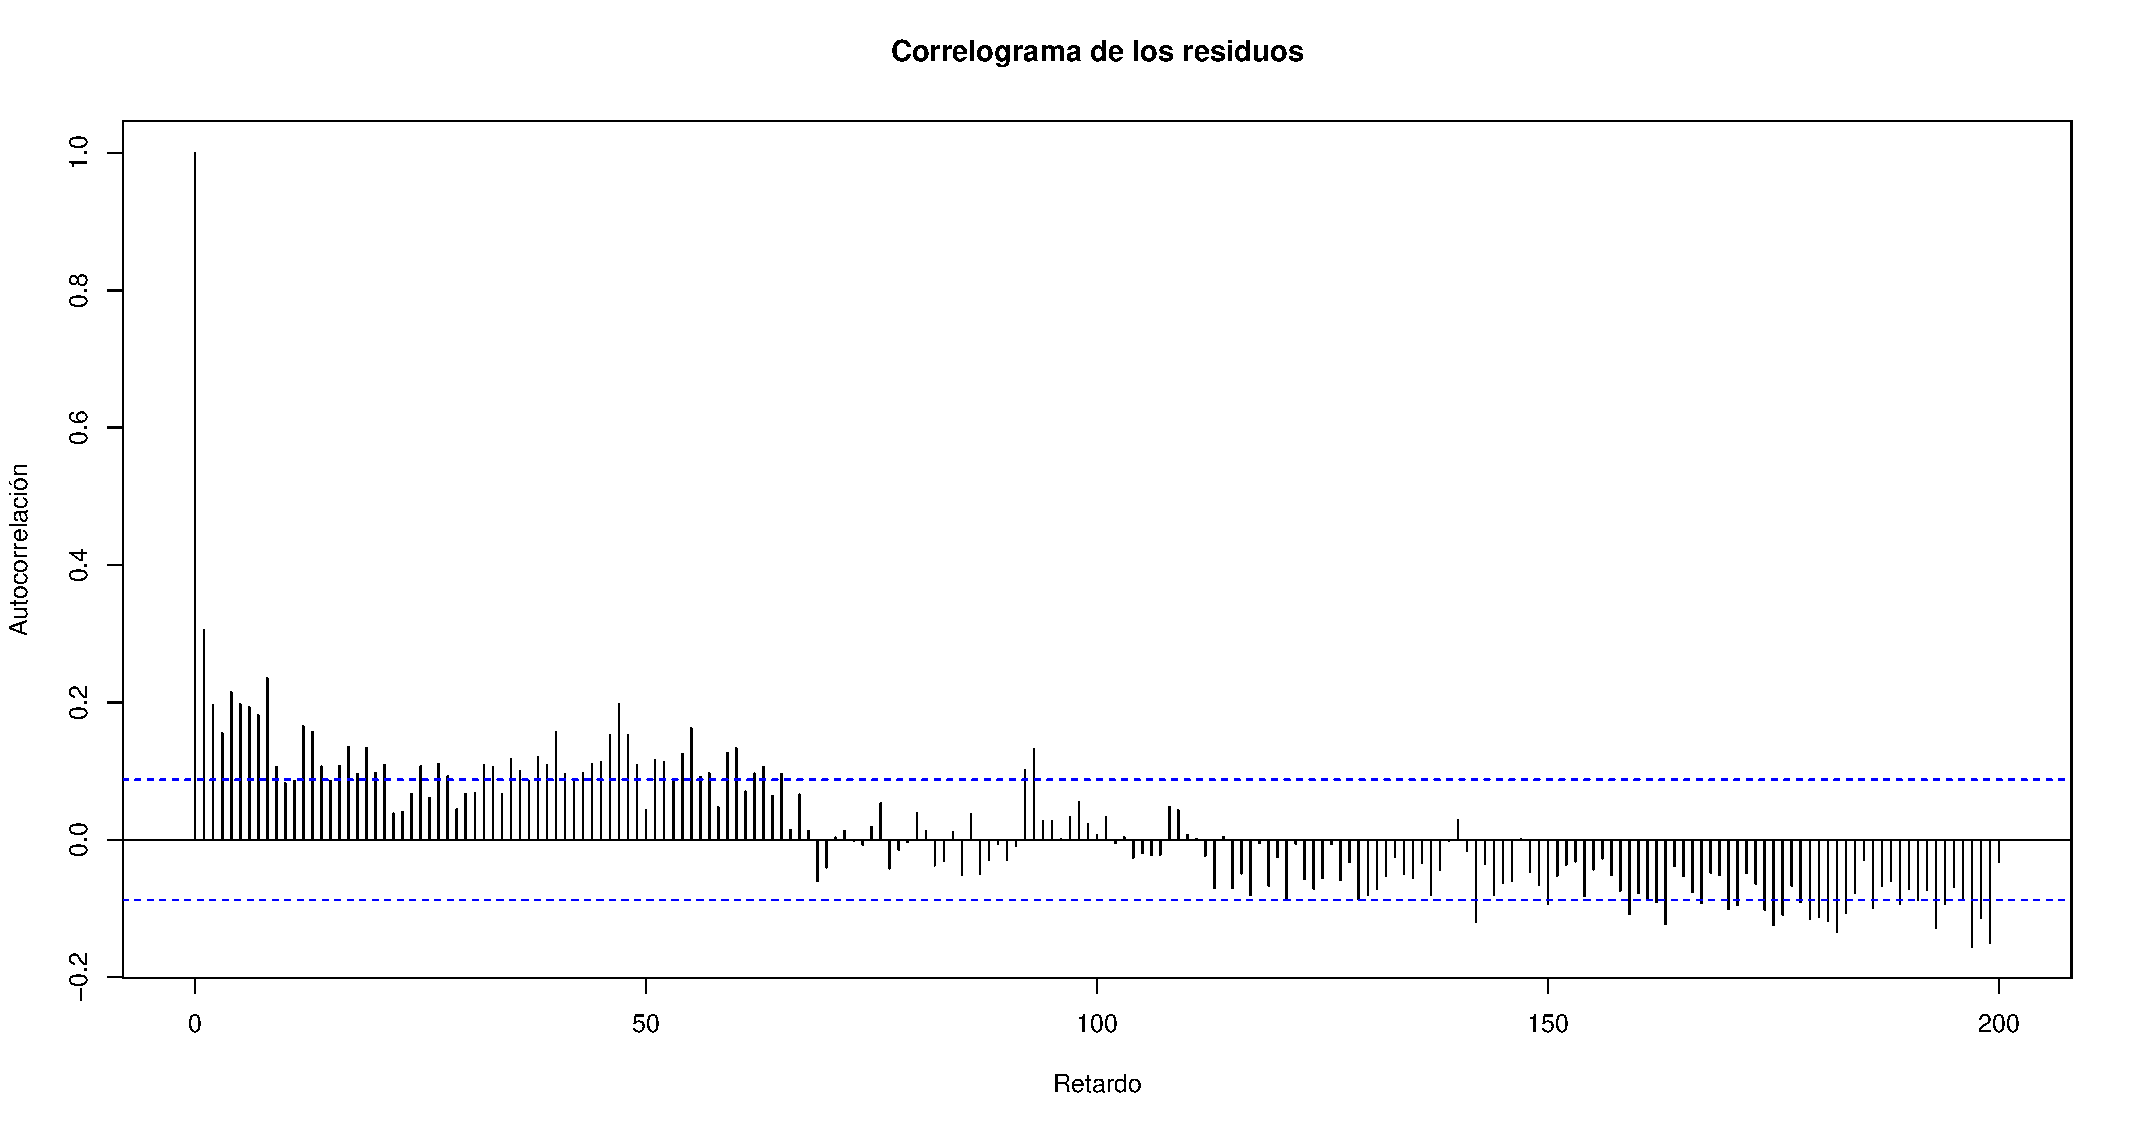
\includegraphics[width=11.8cm]{imagenes/correlograma.pdf}
        \caption{Correlograma de los residuos}
        \label{fig:Densidad}
    \end{center}
\end{figure}
\end{frame}

\begin{frame}
\frametitle{Descripción y resultados de las pruebas aplicadas}
\begin{itemize}
\item Prueba de Rachas:Dada una sucesión de n observaciones de una variable que solo puede tomar dos valores, una racha es una sucesión de uno o más datos con el mismo valor que están seguidos y precedidos por datos con el otro valor, o por ningún dato si se encuentran en el inicio o el final de la sucesión.
~\\ Ejemplo: En la sucesión A BBB AA BB A B se presentan 6 rachas.
~\\ \textbf{Hipótesis:} Las hipótesis que se plantean en esta prueba son:
~\\$H_{0}:$La muestra es aleatoria
~\\$H_{1}:$La muestra no es aleatoria
~\\ \textbf{Estadístico de prueba:} El estadístico de prueba es el número total de rachas, R, en la sucesión.
\end{itemize}
\end{frame}

\begin{frame}
\frametitle{Descripción y resultados de las pruebas aplicadas}
~\\ \textbf{Distribución del estadístico de prueba R:}Su distribución bajo la hipótesis nula $H_{0}$ esta dada por:
~\\$P\left\lbrace{R=r}\right\rbrace=\frac{2\binom{n_{1}-1}{\frac{r}{2}-1}\binom{n_{2}-1}{\frac{r}{2}-1}}{\binom{n_{1}+n_{2}}{n_{1}}}$ si r es par

~\\$P\left\lbrace{R=r}\right\rbrace=\frac{\binom{n_{1}-1}{\frac{r-1}{2}-1}\binom{n_{2}-1}{\frac{r-1}{2}}+\binom{n_{1}-1}{\frac{r-1}{2}}\binom{n_{2}-1}{\frac{r-1}{2}-1}}{\binom{n_{1}+n_{2}}{n_{1}}}$ si r es impar
~\\Para r=2,3,4,...,$n_{1}+n_{2}$
~\\ \textbf{Aproximación a la normal:}
$$Z=\frac{R-\left(\frac{2n_{1}n_{2}}{n_{1}+n_{2}}+1\right)}{\sqrt{\frac{2n_{1}n_{2}(2n_{1}n_{2}-n_{1}-n_{2})}{(n_{1}+n_{2})^2 (n_{1}+n_{2}-1)}}} $$
\end{frame}

\begin{frame}
\frametitle{Descripción y resultados de las pruebas aplicadas}
~\\ \textbf{Región de rechazo:}Se duda de la aleatoriedad cuando hay muchas o muy pocas rachas. Por tanto, la región de rechazo es de la forma:
~\\ $R>R_{n_{1},n_{2};(1-\frac{\alpha}{2})}$ o $R<R_{n_{1},n_{2};\frac{\alpha}{2}}$
~\\Donde la parte derecha de cada inecuación son los percentiles $(1-\frac{\alpha}{2})$ y $\frac{\alpha}{2}$ de la distribución del número de rachas R, cuando hay $n_{1}$ observaciones del tipo A y $n_{2}$ del tipo B.
~\\ \textbf{Resultado:}
\begin{figure}[!h]
    \begin{center}
        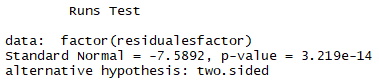
\includegraphics[width=10cm]{imagenes/rachas.png}
        \caption{Resultado prueba de rachas}
        \label{fig:Densidad}
    \end{center}
\end{figure}
\end{frame}

\begin{frame}
\frametitle{Descripción y resultados de las pruebas aplicadas}
\begin{itemize}
\item Prueba de Durbin-Watson: El Test de Durbin-Watson permite evaluar si existe autocorrelación en una Regresión lineal, sea simple o múltiple. Con ello se pretende ver si los valores presentan algún tipo de dependencia en cuanto al orden de obtención. Las hipótesis que se plantean son las siguientes:
~\\$H_{0}:\rho=0$
~\\$H_{1}:\rho\neq 0$
~\\ \textbf{Estadístico de prueba:}El estadístico de Durbin-Watson (D) está condicionado según el orden de las observaciones. El estadístico de Durbin-Watson determina si la correlación entre los términos de error adyacentes es o no es igual a cero. este estadístico esta dado por : $D=\frac{\sum\limits_{t=2}^{n}(e_{t}-e_{t-1})^2}{\sum\limits_{t=1}^{n}e_{t}^2}$ donde $e_{t}$ es el residuo t-esimo o a tiempo t.
\end{itemize}
\end{frame}

\begin{frame}
\frametitle{Descripción y resultados de las pruebas aplicadas}
~\\ \textbf{Región de rechazo:}Para rechazar se utiliza una tabla con lo valores críticos del estadístico, las regiones de rechazo son:
\begin{itemize}
\item Si $d < d_{L,\alpha}$ existe evidencia estadística de que los términos de error estén autocorrelacionados positivamente.
\item Si $d > d_{U,\alpha}$ no hay evidencia estadística de que los términos de error estén autocorrelacionados positivamente.
\item Si $d_{L,\alpha} < d < d_{U,\alpha}$ la prueba no es concluyente.
~\\ \textbf{Resultado:}
\begin{figure}[!h]
    \begin{center}
        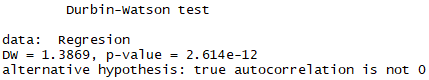
\includegraphics[width=10cm]{imagenes/durbin.png}
        \caption{Resultado de la prueba de Durbin-Watson}
        \label{fig:Densidad}
    \end{center}
\end{figure}
\end{itemize}
\end{frame}

\begin{frame}
\frametitle{Descripción y resultados de las pruebas aplicadas}
\begin{itemize}
\item Prueba de Ljung-Box:La prueba de Ljung-Box es un tipo de prueba estadística que evalúa si un grupo cualquiera de autocorrelaciones de una serie de tiempo son diferentes de cero. En lugar de probar la aleatoriedad en cada retardo distinto, esta prueba la aleatoriedad en general basado en un número de retardos.
~\\En la prueba de Ljung-Box se puede definir o plantear las hipótesis de la siguiente manera:
~\\$H_{0}:$Los datos se distribuyen de forma independiente (es decir, las correlaciones en la población de la que se toma la muestra son 0, de modo que cualquier correlación observada en los datos es el resultado de la aleatoriedad del proceso de muestreo).
~\\$H_{1}:$ Los datos no se distribuyen de forma independiente.
\end{itemize}
\end{frame}

\begin{frame}
\frametitle{Descripción y resultados de las pruebas aplicadas}
~\\ \textbf{Estadístico de prueba:} El estadístico de prueba es: $Q=n(n+2)\sum\limits_{k=1}^{h}\frac{\hat{\rho_{k}^{2}}}{n-k}$
~\\ donde n es el tamaño de la muestra, $\displaystyle {\hat {\rho }}_{k}$  es la autocorrelación de la muestra en el retraso k y h es el número de retardos que se están probando.
~\\ \textbf{Región de rechazo:} Para un nivel de significancia $\alpha$ la región critica para rechazar la hipótesis de aleatoriedad es: $Q>\chi^{2}_{1-\alpha,h}$
~\\donde $\displaystyle \chi _{1-\alpha ,h}^{2}$ es el $\alpha$-cuantil de la distribución chi-cuadrado con m grados de libertad.
\end{frame}

\begin{frame}
\frametitle{Descripción y resultados de las pruebas aplicadas}
~\\ \textbf{Resultado:}\begin{figure}[!h]
    \begin{center}
        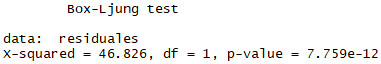
\includegraphics[width=10cm]{imagenes/box.png}
        \caption{Resultado de la prueba de Ljung-Box}
        \label{fig:Densidad}
    \end{center}
\end{figure}
\end{frame}

\begin{frame}
\frametitle{Conclusión sobre nuestro modelo ajustado}
~\\Teniendo en cuenta las pruebas aplicadas, donde vimos que en la prueba gráfica, muchas barras se nos salen de los intervalos y en las pruebas estadísticas los p valores de las tres pruebas son demasiado bajos llevándonos a rechazar siempre $H_{0}$, concluyendo que los residuos no son independientes, lo más común y razonable es concluir que nuestro modelo ajustado no cumple con este supuesto de independencia en los errores, por lo cuál diríamos que lo recomendable sería no usar este modelo. Sin embargo, los errores podrían ser independientes aún cuando los residuos no lo sean, y el supuesto se hace para los errores mas no para los residuos, pero eso no hay forma de probarlo a ciencia cierta, sin embargo hay que tener muy en cuenta los resultados obtenidos y queda a criterio de la persona si ignora estos resultados.
\end{frame}


\end{document}